
\begin{frame}
	\frametitle{Ecuación Logística}
	\begin{empheq}[box=\shadowbox*]{align*}
		dy(t)& = \lambda y(t) ( K - y(t) )dt+ \sigma y(t)^{\alpha}| K  - y(t) |^\beta dW_t\\
		X_0& = 50, 
		K = 1000, 
		\alpha = 1,
		\beta = \num{0.5}, 
		\lambda = 0.25, 
		\rho = 0,
		\sigma = \num{0.05}
	\end{empheq}
%
	\begin{columns}
		\column{.6\textwidth}
		\begin{overlayarea}{1.0\textwidth}{\textheight}
			\only<2->{
				\begin{center}
					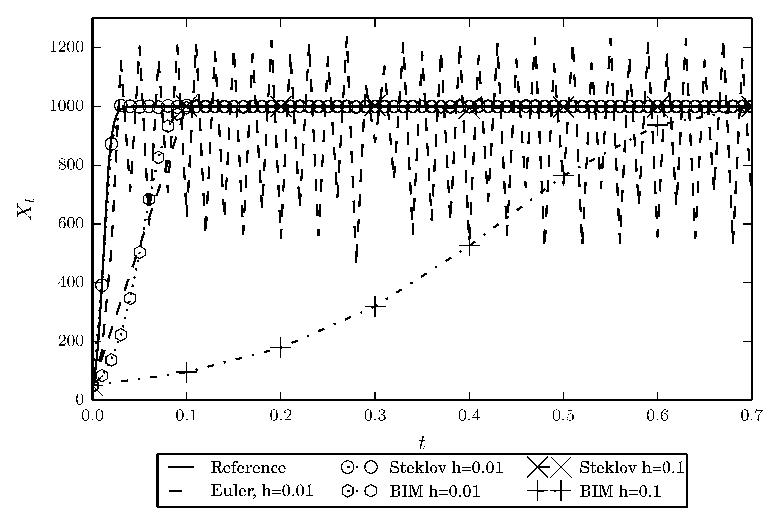
\includegraphics[scale=.5]{images/LogisticSDE.eps}
				\end{center}
			}
		\end{overlayarea}
		\column{.4\textwidth}
			\begin{overlayarea}{1.0\textwidth}{\textheight}
				\begin{bibunit}[apalike]
					\nocite{Schurz2007}
					\only<2>{
						\biblio{BibliografiaTesis}	
					}
				\end{bibunit}
			\end{overlayarea}
	\end{columns}	
\end{frame}
%%%%%%%%%%%%%%%%%%%%%%%%%%%%%%%%%%%%%%%%%%%%%%%%%%%%%%%%%%%%%%%%%%%%%%%%%%%%%%%%%%%%%%%%%%%%
\begin{frame}%[label=frm:20]
	\frametitle{Din\'amica Browniana}
	%
	\begin{overlayarea}{1.0\textwidth}{.15\textheight}
		\begin{empheq}[box=\shadowbox*]{equation*}
				dX_t= -X_t^3 +\xi dB_t,
			\qquad Dta=\num{e-6}
		\end{empheq}
	\end{overlayarea}
	%
	\begin{overlayarea}{1.0\textwidth}{.89\textheight}
		\only<2->{
			\begin{center}
				\includegraphics[scale=.5]{images/short-longMSD.eps}
			\end{center}
		}
		\begin{bibunit}[apalike]
			\nocite{Braanka1998}
			\only<2>{
				\biblio{BibliografiaTesis}
			}
		\end{bibunit}
	\end{overlayarea}
\end{frame}